\documentclass{article}
\usepackage{{amsfonts}}
\usepackage[a4paper, total={6in, 8in}, margin={1in}]{geometry}
\usepackage{{mathtools}}
\usepackage{amsmath}
\usepackage{xcolor}
\usepackage{multicol}

\usepackage{graphicx}
\graphicspath{ {./graphics/}}
\usepackage{epstopdf}

\author{James Lounds}
\title{Remedial Math 111 Group Project}

\begin{document}

\maketitle
\newpage

\section{Task 1}
\subsection{Brief}
The Royal Mint wants to perform an investigation on the optimal production of each denomination of coin.
\newline
I need to:
\begin{itemize}
    \item calculate the change given for each transaction under £1,

    \item calculate the distribution of the number of coins given as change,
    \item calculate the consequences of removing the 20p coin from circulation,
    \item discuss the consequences of removing the 1p and 2p coins from circulation.
\end{itemize}
\subsection{Solution}
I needed to define a few functions in MATLAB to make these calculations possible.
\begin{itemize}
    \item coins\_counts

          has arguments
          \begin{itemize}
              \item prices - vector of prices to count change for
              \item coins - the vector of the coins we have (unlimited) access to
          \end{itemize}

          returns
          \begin{itemize}
              \item counts - a matrix with columns corresponding to how many of each type of coin are in the optimal change give.
          \end{itemize}
    \item coin\_occurence\_table

          has arguments
          \begin{itemize}
              \item prices - vector of prices to count change for
              \item coins - the vector of the coins we have (unlimited) access to
          \end{itemize}

          returns
          \begin{itemize}
              \item table - a table with the number of times a coin was used in the optimal change for each price
          \end{itemize}
    \item coin\_number\_distribution\_table

          has arguments
          \begin{itemize}
              \item prices - vector of prices to count change for
              \item coins - the vector of the coins we have (unlimited) access to
          \end{itemize}

          returns
          \begin{itemize}
              \item table - a table with the expected value of each denomination being used in the optimal solutioin of a price in prices
          \end{itemize}
\end{itemize}
I then used a helpful tool developed by Víctor Martínez to convert the tables to \LaTeX
\subsection{Results}
For the standard set of coins $ \{50p, 20p, 10p, 5p, 2p, 1p \} $ and prices $ \{0, 1, 2, \ldots, 99 \} $
\\ \\
\begin{tabular}{cc}

    \begin{tabular}[t]{llll}
        Denomination & 0  & 1  & 2  \\
        \hline
        50           & 50 & 50 & 0  \\
        20           & 40 & 40 & 20 \\
        10           & 60 & 40 & 0  \\
        5            & 50 & 50 & 0  \\
        2            & 40 & 40 & 20 \\
        1            & 60 & 40 & 0  \\
        \hline
    \end{tabular}
    \: \: \:

    \begin{tabular}[t]{ll}
        Occurences & Probability (\%) \\
        \hline
        0          & 1                \\
        1          & 6                \\
        2          & 17               \\
        3          & 28               \\
        4          & 28               \\
        5          & 16               \\
        6          & 4                \\
        \hline
    \end{tabular}
\end{tabular}
\\ \\ \\
For the set of coins without 1p and 2p $ \{50p, 20p, 10p, 5p \} $ and prices $ \{ 0, 5, 10, \ldots, 95 \} $
\\ \\
\begin{tabular}{cc}
    \begin{tabular}[t]{llll}
        Denomination & 0  & 1  & 2 \\
        \hline
        50           & 20 & 0  & 0 \\
        20           & 20 & 0  & 0 \\
        10           & 10 & 10 & 0 \\
        5            & 10 & 10 & 0 \\
        \hline
    \end{tabular}
    \: \: \:
    \begin{tabular}[t]{ll}
        Occurences & Probability (\%) \\
        \hline
        0          & 25               \\
        1          & 50               \\
        2          & 25               \\
        \hline
    \end{tabular}
\end{tabular}

\subsection{Conclusions}
Our current coin system is reasonably well designed to pay for any natural value of pennies.
If we were to limit transactions to multiples of five pence, we would be able to substantially reduce the number of coins needed to pay.
However, this is not without consequence.
There is a significant psychological aspect to pricing.
Many shops will price things one penny under a whole price.
This is purported to reduce the percieved cost in the customers' minds.
If we were to force more quantized pricing, this psychological aspect may be reduced.
Nonetheless, given the increase in purchases via non-cash methods, it would not be infeasible for retailers to round up or down to the nearest 5 pence.
Cash is not free to handle, and can be more expesive than the fees cards processors charge.
By reducing the amount of small change, the average value of the cash increases, thus decreasing the relative cost of handling cash.
\newpage
\subsection{Code}
\subsubsection{task\_1.m}
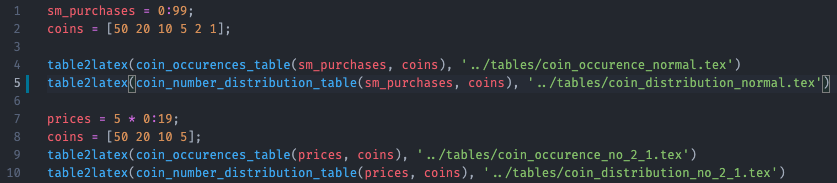
\includegraphics[width=\textwidth]{task_1/task_1.m.png}
\\
This code only invokes the previously defined functions for our paramterers and puts the tables in TeX files.

\subsubsection{coin\_occurences\_table.m}
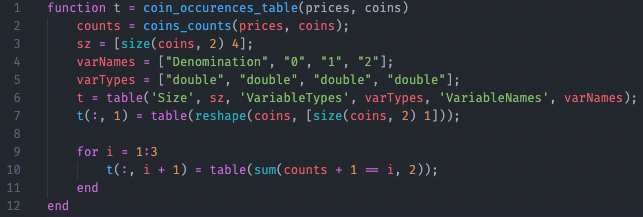
\includegraphics[width=\textwidth]{task_1/coin_occurences_table.m..png}
\\
This function produces a table ofthe number of times each coin is used over the 99 transactions.
Lines 2-6 initialise the table, while the remaining lines iterate up to the (hardcoded) maximum number of times a coin can be used optimally.


\subsubsection{coin\_number\_distribution\_table.m}
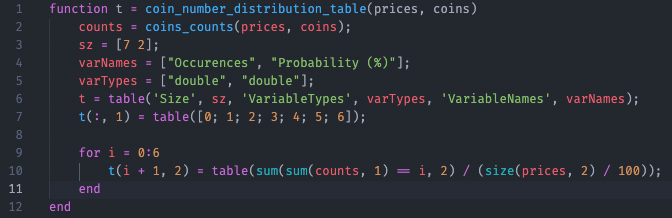
\includegraphics[width=\textwidth]{task_1/coin_number_distribution_table.m.png}
This function is very similar to the previous, but instead calculates the expected value of the number of each coin used in some optimal change.

\subsubsection{coins\_counts}
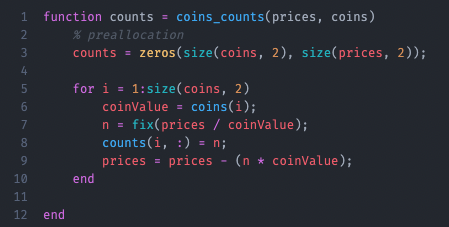
\includegraphics[width=\textwidth]{task_1/coins_counts.m.png}
\\
This function calculates a matrix with each entry being the number of coins of the denomination (indicated by the row) needed for the optimal change for the price (indicated by the column).
It does this by iterating through each price, and appending the correct coin count vector to the end of the counts matrix.
Each entry in the column vector is calculated by floor division, then leaving the remainder for the next iteration.
\newpage
\section{Task 2}
\subsection{Brief}
The price of gold bullion can be modelled using Random Walk Theory.
If Party A has £6 and Party B has £14, and they were to play a game where a fair coin was flipped, and the winner gave the loser £1, this would produce a random walk.
I need to calculate:
\begin{itemize}
    \item The probability Part A wins.
    \item The probability that Party A loses given that they were within £1 of winning.
\end{itemize}
\subsection{Solution}
I defined only one function in my solution:
\begin{itemize}
    \item play\_game \\
          has arguments
          \begin{itemize}
              \item initial\_scores - the amount of money A and B have at the start, as a row vector.
          \end{itemize}
          returns
          \begin{itemize}
              \item scores - a matrix where each row is the amount of money A and B have after a round.
          \end{itemize}
\end{itemize}
\newpage
\subsection{Results}
\begin{tabular}{ll}
    Probability A Wins & Probability A Loses Closely \\
    \hline
    0.2978             & 0.015                       \\
    \hline
\end{tabular} \\ \\
Note: only the bottom two plots have scale 0-20. Teh bottom left plot is a close loss for A\\
\begin{figure}[h!]
    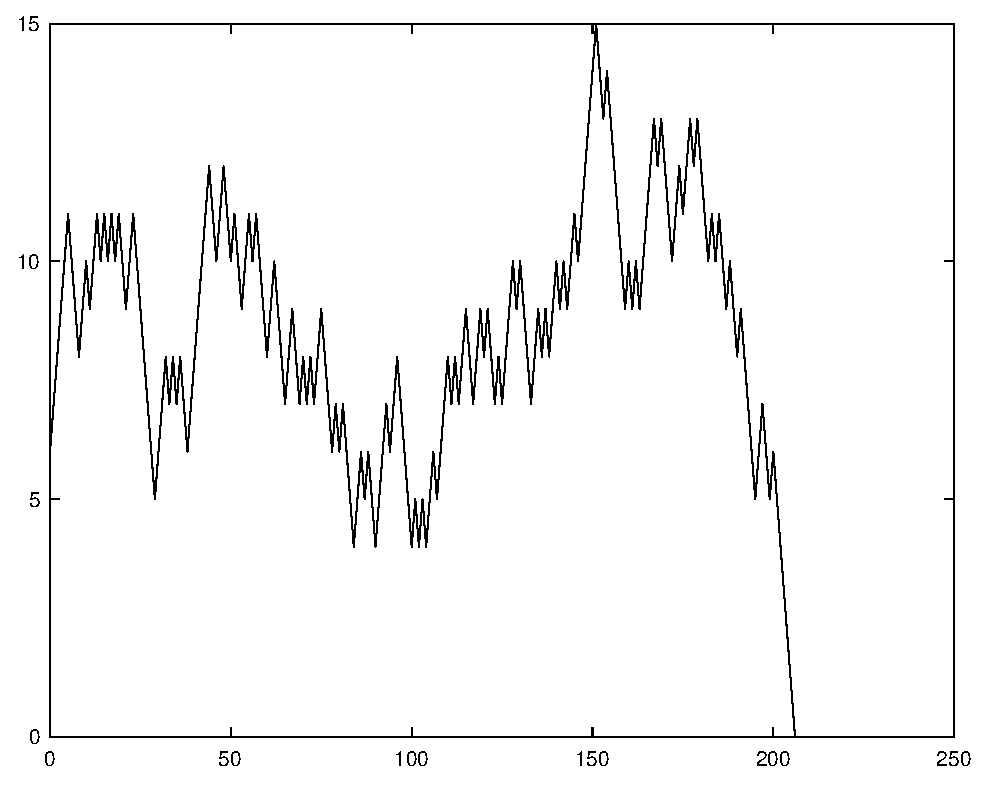
\includegraphics[width=.5\linewidth]{A_loss_1}
    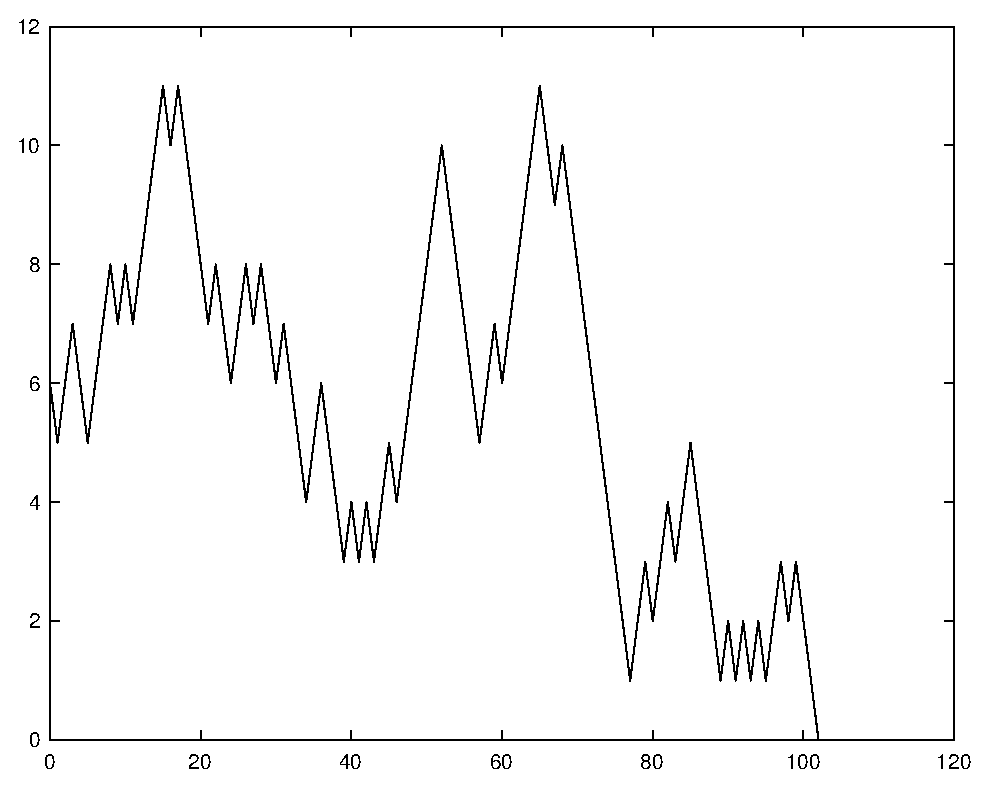
\includegraphics[width=.5\linewidth]{A_loss_2}
    \\\\
    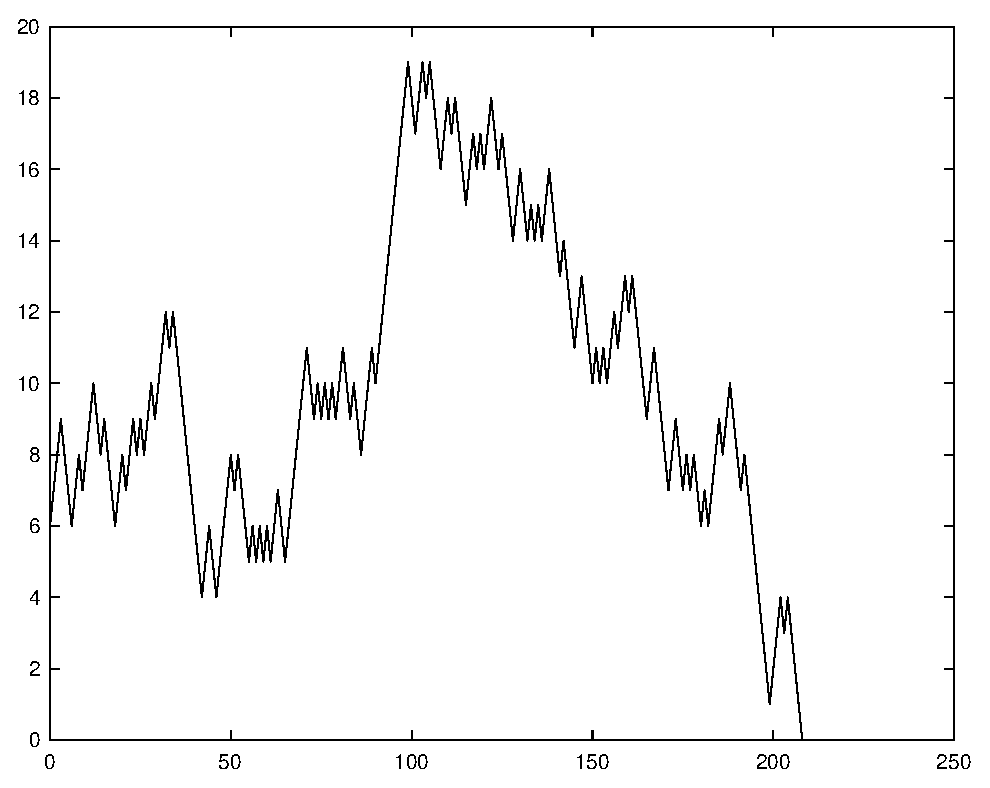
\includegraphics[width=.5\linewidth]{close_loss}
    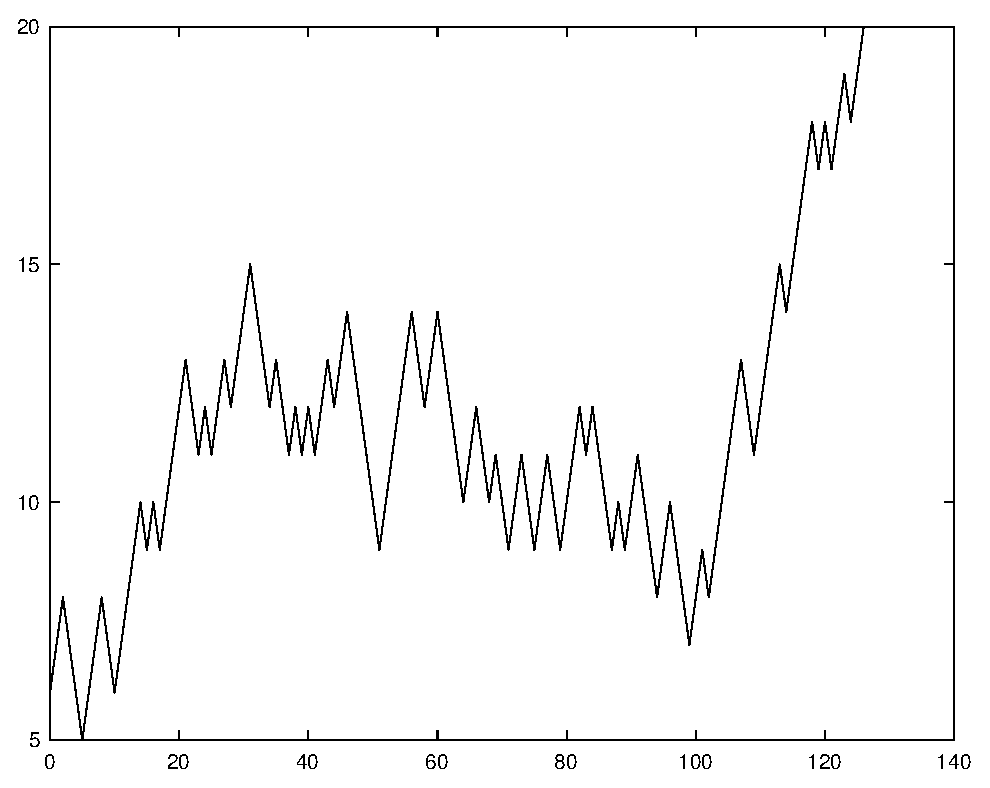
\includegraphics[width=.5\linewidth]{A_win_1}
\end{figure}



\newpage

\subsection{Code}
\subsubsection{play\_game.m}
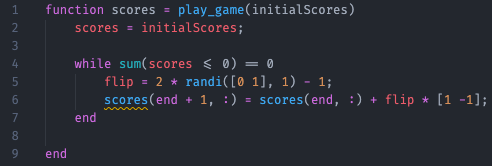
\includegraphics[width=\textwidth]{task_2/play_game.m.png}
This code loops until either player has a score of 0. On each iteration, it generates a flip $\in \{-1, 1\}$.
It then adds a new row to the end of the scores matrix, with each playeer's score incremented or decremented depending on the value of flip.

\subsubsection{task\_2.m}
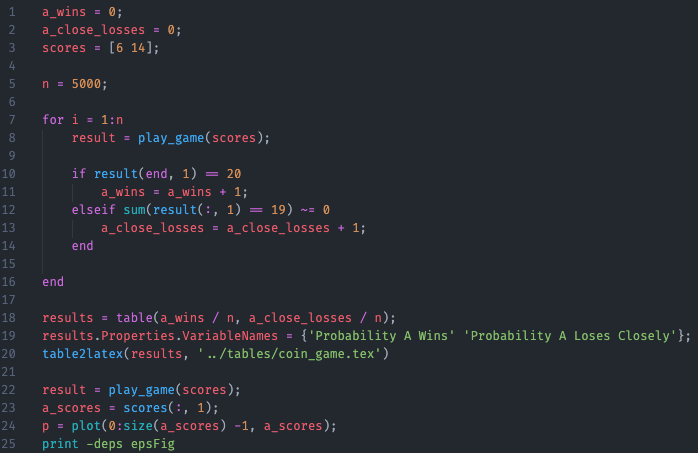
\includegraphics[width=\textwidth]{task_2/task_2.m.png}
We start by initialising some variables.
We then play $n$ random games and record if A won, or if A closely lost.
This data is stored in a table then exported to \LaTeX.
We then run one more random game, which is plotted, and then exported to \LaTeX

\end{document}